%%%%%%%%%%%%%%%%%%%%%%%%%%%%%%%%%%%%%%%%
% Chapter 5: Proof-of-concept: Synthetic Dutch Homicide Data
%%%%%%%%%%%%%%%%%%%%%%%%%%%%%%%%%%%%%%%%

\label{proofofconcept}

In order to showcase the applied use, advantages and limitations of synthetic data, this chapter will elaborate on the generation of a synthetic dataset based on the Dutch Homicide Monitor. This proof-of-concept covers the entire process of synthetic data generation (as described in Chapter 4), from data preprocessing and model selection to the generation and evaluation of synthetic data, using step-by-step discussions on the choices made during that process. 

\section{Dataset: The Dutch Homicide Monitor}

The Dutch Homicide Monitor is a dataset administered by researchers at Leiden University in the Netherlands (authors of this report). Through 25 nuclear attributes, the dataset captures detailed information on homicides committed in the Netherlands, including case-level information (such as the time of day and type of crime scene) as well as individual-level data of victims and (suspected) perpetrators, such as the age, gender, occupation and country of birth. The information included in the Dutch Homicide Monitor is derived from six sources: public sources, such as the annual homicide list collected by Elsevier Magazine, news articles and public court ruling, as well as non-public sources, such as police data, information from the public prosecution service and forensic records. As of June 2024, the Dutch Homicide Monitor captures all homicide committed between 1992 and 2023, which covers 5563 cases, and information on 5920 victims and 7542 (suspected) perpetrators. 

\textbf{Structure of the data}\\
The Dutch Homicide Monitor consists of 25 nucleus variables. Most of these variables (21) are categorical; only four variables (number of victims, number of perpetrators, age, date, description of incident) are non-categorical. Categories within a variable range from two (male/female) to 35 categories (victim-perpetrator relationship). In addition to these 25 variables, the dataset has three variables that act as identifying variables: a case number (which represents a case), a serial number (which represents each individual) and a variable that identifies one principal victim and perpetrator (if known) per case. These variables are defined in a \href{https://www.universiteitleiden.nl/binaries/content/assets/governance-and-global-affairs/isga/dfvm---coding-manual-marieke-liem.pdf}{coding manual}, which is shared with other researchers in the European Homicide Monitor network. Furthermore, in order to allow cross-matching between multiple data sources, the address at which the homicide took place, the name and the social security number of the victim and perpetrator are included as additional variables.

\vspace{10pt}
\begin{table}[H]
\small
\centering
\begin{tabular}{@{}ll@{}}
\toprule
Case-level                  & Individual-level                 \\ \midrule
Case number                 & Serial number                    \\
Description                 & Crimescene                       \\
Number of victims           & Modus operandi                   \\
Number of perpetrators      & Type: victim or perpetrator?     \\
Spatial region              & Gender                           \\
City                        & Age                              \\
Year homicide was committed & Profession                       \\
Date of homicide            & Country of birth                 \\
Time of day                 & Alcohol (ab)use                  \\
                            & Drug (ab)use                     \\
                            & Violent history                  \\
                            & Context of homicide              \\
                            & Victim-perpetrator relationship  \\
                            & Main motive of perpetrator       \\
                            & Suicide (attempt) by perpetrator \\
                            & Stage in judicial system         \\ \bottomrule
\end{tabular}
\caption{Variables included in Dutch Homicide Monitor}
\label{tab:my-table}
\end{table}
\vspace{10pt}


The variables are embedded in the columns. Each record in that dataset represents an individual - either a victim or (suspected) perpetrator of the homicide. A variable 'Type' classifies the individual as either a victim or perpetrator. One homicide case can involve multiple victims and/or perpetrators, meaning that one case can span from two to six or even ten rows. Information stored on case-level variables is the same across the rows that belong to the same case, whereas individual-level information can vary for each row. 

\vspace{10pt}
\begin{table}[H]
\small
\centering
\begin{tabular}{@{}lllllll@{}}
\toprule
Case number & Serial number & Time of day & Type        & Gender & Age & .. \\ \midrule
1           & 1.1           & 6am-12pm    & Victim      & F      & 22  & .. \\
1           & 1.2           & 6am-12pm    & Perpetrator & M      & 24  & .. \\
2           & 2.1           & 6pm-12am    & Victim      & M      & 46  & .. \\
2           & 2.2           & 6pm-12am    & Perpetrator & M      & 55  & .. \\
2           & 2.3           & 6pm-12am    & Perpetrator & M      & 43  & .. \\ \bottomrule
\end{tabular}
\caption{Example of DHM structure}
\label{tab:my-table}
\end{table}
\vspace{10pt}

\subsection{Privacy of homicide data in the Dutch Homicide Monitor}
The Dutch Homicide Monitor contains sensitive personal information on victims and (suspected) perpetrators of homicide in the Netherlands. Specifically sensitive information includes the gender, age, country of birth, occupation, address of the incident and more. Although some of this information can be found in public sources, such as news articles, overall, this information is protected through the European Union's GDPR regulation, as well as agreements made with the Dutch National Police and Public Prosecution Office of the Netherlands on the handling of their data. The sensitive nature of the data limits the use of the Dutch Homicide Monitor: students, journalists or other researchers who want to use the disaggregated dataset need to apply for access to the data which requires approval by the Dutch National Police.This process can take up considerable time and efforts, making it infeasible for certain use case. In addition, implementing FAIR standards to the dataset is limited, given that the dataset is neither accessible, interoperable, nor reusable. 

%%%%%%%%%%%%%%%%%%%%%%%%%%%%%%%%%%%%%%%%

\section{Generating a synthetic version of the Dutch Homicide Monitor}

\subsection{First attempt}

To begin with, we set a list of requirements for the to-be-generated synthetic dataset. We want a: 

\begin{enumerate}[label=\alph*)]
	\item fully synthetic dataset
	\item dataset with the same structure as the original data that allows for analysis on case-, victim- and perpetrator-level
	\item statistical accuracy that allows for replication of previous studies using the original data
	\item safeguarding of sensitive information to adhere to GDPR and additional regulations associated with the original data
\end{enumerate}

Through these requirements, we aimed to generate a synthetic dataset that is complete and can be used for several purposes, such as student exercises, as a source of information for journalists and other stakeholders, as well as a source for future academic studies. In short, a dataset that can be registered and used for any possible future purpose.

\textbf{Step 1: Preparations} \\
Given that the requirements do not ask for much changes to the original data, the preparations were minimal. As with any data analysis, we checked the data for internal inconsistencies, for accidental mistakes in the coding (e.g. 998 instead of 999), duplicates and so on. In addition, we excluded three identifying variables: the name and social security number of victims and (suspected) perpetrators and the address of the homicide. Although these variables could be synthesised, they would carry no meaning in the synthesised dataset, but may increase the risk for privacy breaches. The identifying variables (case number, serial number and the variables that differentiate victims from perpetrators) have been kept in the to-be-synthesised dataset.

Another concern during this phase was data quality. The fraction of missing data for certain cases can be high, e.g. due to a lot of missing information in the homicide, such as the identity of the perpetrator, or due to a lack of details in the available data sources. For example, police reports on earlier homicides may not have as much detail as police reports on more recent cases. In order to have a high-quality synthetic dataset of the Dutch Homicide Monitor, we decided to create a dataset that only contains ten years of homicide data. The chosen ten years of data have the highest data quality in the Dutch Homicide Monitor. After extracting these ten years of high-quality data from the Dutch Homicide Monitor, the new and to-be-synthesised dataset contained 1271 cases, and information on 1348 victims and 1711 (suspected) perpetrators. 

Finally, we determined two logical dependencies in our dataset that are present in the original data and would need to be replicated in a synthetic dataset. First, we determined that any homicide victim involved in a \textit{child homicide} needed to be \textit{younger than 17 years}. Another logical dependency in the original data is between the type of homicide and victim-perpetrator relationship. Specifically, we determined that homicides categorized as intimate partner homicides needed to co-occur with the victim-perpetrator relationship of \textit{partner} or \textit{ex-partner}.

\textbf{Step 2: Choosing generation method and tool} \\
The choice of generation method and tool was determined by two factors: First, the generation method needed to fit the structure of our data. Second, the generation method and tool specifically needed to be easy to use, as the goal of the project and this guide on synthetic data was to make synthetic data accessible to a broader audience without extensive knowledge of computations or data science. Therefore, we evaluated the extent of helpful and guiding documentation for each generation method and tool and selected a member of the project team with no experience with synthetic data as the lead for the generation process. Following the principals of open science, only open-source tools (thus no commercial options) were included in the decision process.

As mentioned in Section 3.1, three main categories of synthetic data generation methods can be distinguished: rule-based, statistical, and machine learning methods. We opted for a statistical method as rule-based methods are time-consuming to develop and rely heavily on prior domain knowledge, and our dataset is relatively small to justify using advanced machine learning methods like GANs and VAEs. An additional benefit of statistical methods over machine learning methods are increased interpretability of the generation process. To generate high-utility synthetic data, the statistical method should not only capture univariate distributions, but also dependencies between variables. An apt statistical method are thus copula models, which separately model univariate distributions and the dependency structure between variables, after which they are linked together to model the multivariate dataset \cite{nelsen2006introduction}.

Several tools use copulas as a basis for the synthesis of data. Yet, the structure of our data limited the options of tools available to us, given that not all tools are equipped to synthesise data with dependencies across rows and columns. After reviewing several options, we decided that the best approach to keep these dependencies would be through a multi-table synthesis. In this process, several tables linked through a common id are synthesised whilst keeping the relationships between the tables and variables. In order to prepare our data for this process, we divided the main dataset into three separate ones: one that includes four case-level variables, one that includes thirteen variables containing information on the victims and one that includes twelve variables related to information on the perpetrator. Some variables in the victim- and perpetrator-tables overlap, such as age, gender, country of birth or occupation. 

\vspace{10pt}
\begin{table}[h!]
\small
\centering
\begin{tabular}{@{}lll@{}}
\toprule
Case variables              & Victim variables                & Perpetrator variables            \\ \midrule
Case number                 & Serial number                   & Serial number                    \\
Description                 & Gender                          & Gender                           \\
Number of victims           & Age                             & Age                              \\
Number of perpetrators      & Profession                      & Profession                       \\
Spatial region              & Country of birth                & Country of birth                 \\
City                        & Alcohol (ab)use                 & Alcohol (ab)use                  \\
Year homicide was committed & Drug (ab)use                    & Drug (ab)use                     \\
Date of homicide            & Violent history                 & Violent history                  \\
Time of day                 & Crimescene                      & Main motive                      \\
                            & Modus operandi                  & Suicide (attempt) by perpetrator \\
                            & Context of homicide             & Stage in judicial system         \\
                            & Victim-perpetrator relationship &                                   \\ \bottomrule       
\end{tabular}
\caption{DHM variables split by related case-, victim- or perpetrator-level}
\label{tab:my-table}
\end{table}
\vspace{10pt}

The Synthetic Data Vault (SDV) is one of the very few open-source tools that allow for multi-table synthesis. In addition, it provides extensive documentation and support, which is why we chose the SDV for the synthesis of our homicide dataset. The SDV runs on Python and includes suggestions and requirements for data preparation for the synthesis of multi table data. Our data fulfilled most of the requirements, with the exception of a document/object that defines the meta data across the tables - in other words a document that provides information about the type of data, the id-variables that link the tables together and specific connections between the tables. This information can be set-up manually, following instructions in the SDV-documentation, but the SDV-package also comes with functions that can automatically detect this information from your tables, but these require additional verification and checks.

After following the required steps, our homicide dataset was split into one parent table (in our case, the table with case-level variables) and two child tables (one victim table, one perpetrator table). In this meta-data, the case number is identified as an id that connects the inter-dependent rows across those three tables. 

\vspace{10pt}
\begin{figure}[H]
    \centering
    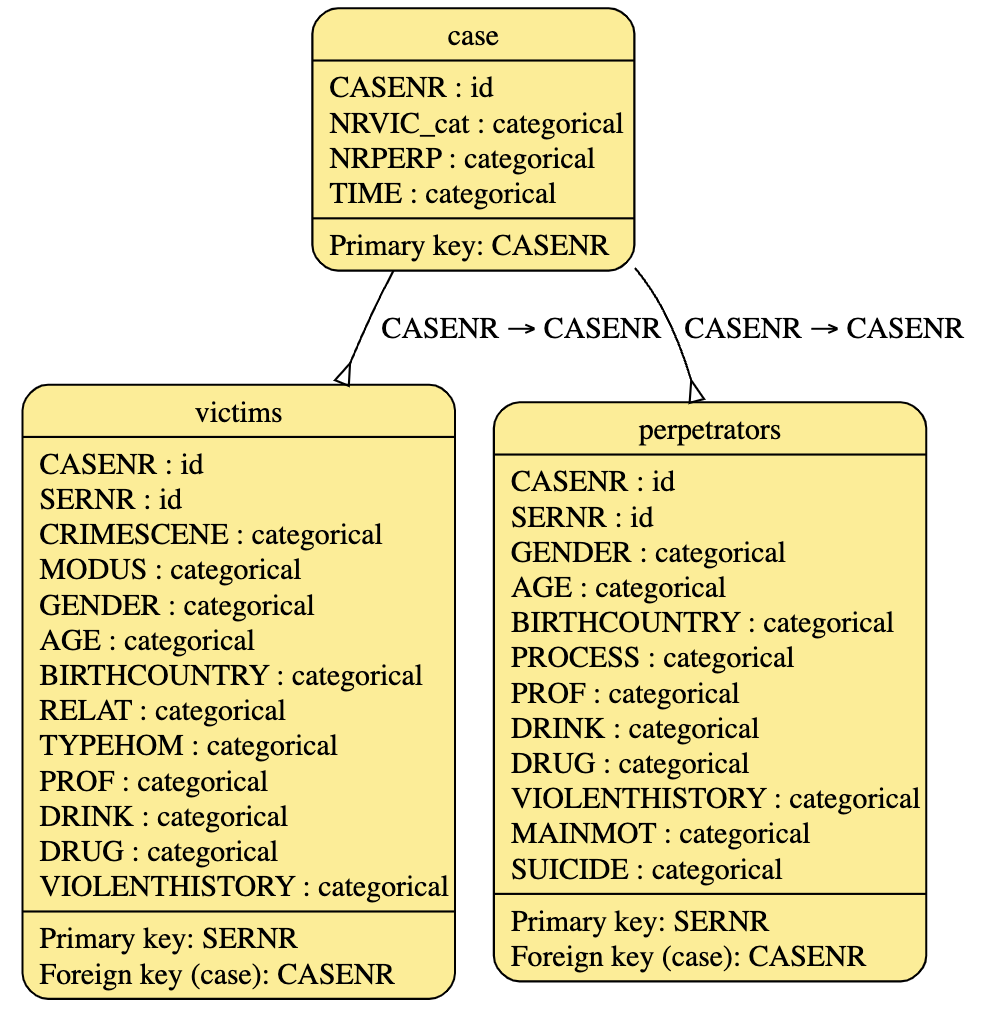
\includegraphics[width=0.6\textwidth]{Images/meta1.png}
    \caption{Dutch Homicide Monitor split into three separate datasets: cases, victims \& perpetrators}
    \label{fig:proof_1}
\end{figure}
\vspace{10pt}

In addition, we prepared the logical dependencies as identified in the preparation phase. Therefore, we wrote a code (available on Github) that would force the model during the synthetic data generation to adhere to the rules set out about the dependency of child homicide and victim age, as well as between intimate partner homicide and victim-perpetrator relationship.

\textbf{Step 3: Generation of synthetic data} \\
The meta-data information prepared in the previous step is then used to create a synthesiser, that is an object that creates synthetic data. The meta-information provides the synthesiser with the relevant information about the structure of the original data, such as the number of columns or categories within a variable. This structure determines the desired structure of the synthetic dataset. After, we loaded the original data into this synthesiser through which it can learn about the patterns and relationships between the variables in our dataset. Finally, the synthesiser generates a synthetic dataset using the structure and identified relationships. We chose to generate as many cases as are included in the original dataset. \\

\vspace{10pt}
\begin{lstlisting}[caption={Synthetic Data Generation: First Attempt}, label={lst:gen_first}]
from sdv.multi_table import HMA Synthesizer

synthesizer = HMASynthesizer(metadata, #this creates a model that knows the structure of the original dataset
                             locales=['nl_NL'] #this generates city names in Dutch

synthsizer.add_constraints(constraints=[
    infanticide_constraint, IPH_constraint
])

synthesizer.fit(DHM) #this tells the model to learn from our original dataset
synthetic= synthesizer.sample(scale=1) #this tells the model to create a synthetic dataset with as many rows as the original dataset
\end{lstlisting}
\vspace{10pt}

The result are three synthetic tables that together form the first synthetic version of the Dutch Homicide Monitor.

\vspace{10pt}
\begin{table}[]
\small
\begin{tabular}{@{}llll@{}}
\midrule
Case number   & Number of victims & Number of perpetrators & Time of day \\ \midrule
sdv-id-nFatwl & 1                 & 1                      & 6am-12am    \\
sdv-id-MulxVy & 1                 & 1                      & 12pm-6pm    \\
sdv-id-gzVJSQ & 2                 & 2                      & 12pm-6pm    \\
...           & ...               & ...                    & ...    \\ \bottomrule    
\end{tabular}
\caption{Synthetic case dataset (first three cases)}
\label{tab:my-table}
\end{table}
\vspace{5pt}

\begin{table}[]
\small
\begin{tabular}{@{}llllll@{}}
\toprule
Case number   & Serial number & Modus operandi              & Gender  & Age     & ... \\ \midrule
sdv-id-nFatwl & sdv-id-fgFyn  & Firearm                     & Missing & 65      & ... \\
sdv-id-MulxVy & sdv-id-MwbyTx & Missing                     & Missing & Missing & ... \\
sdv-id-gzVJSQ & sdv-id-cQNzXJ & Knife or other sharp object & Male    & Missing & ... \\
sdv-id-gzVJSQ & sdv-id-xgDRmZ & Knife or other sharp object & Missing & 24      & ... \\
...           & ...           & ...                         & ...     & ...     & ... \\ \bottomrule
\end{tabular}
\caption{Synthetic victim dataset (associated with first three cases)}
\label{tab:my-table}
\end{table}

\vspace{5pt}
\begin{table}[]
\small
\begin{tabular}{@{}llllll@{}}
\toprule
Case number   & Serial number & Gender & Age & Country of birth & ... \\ \midrule
sdv-id-nFatwl & sdv-id-Edlwqz & Male   & 19  & Missing          & ... \\
sdv-id-MulxVy & sdv-id-LWxGTc & Male   & 17  & Missing          & ... \\
sdv-id-gzVJSQ & sdv-id-imlpGf & Male   & 38  & Netherlands      & ... \\
sdv-id-gzVJSQ & sdv-id-UlNuoi & Male   & 24  & Netherlands      & ... \\
...           & ...           & ...    & ... &                  & ... \\ \bottomrule
\end{tabular}
\caption{Synthetic perpetrator dataset (first three cases)}
\label{tab:my-table}
\end{table}
\vspace{10pt}

\textbf{Step 4: Privacy and Utility Evaluation} \\ 
With regards to the utility, the generated synthetic dataset was of moderate quality.
The SDV package offers several options within the package to evaluate the quality of the synthetic data. First, one can run diagnostics on the synthetic data structure and validity, which test whether the synthesiser adhered to the categories of the original dataset, that variables classified as id have unique numbers for each row and that all of the variables have been adapted into the synthetic dataset. In our synthetic dataset, both statistics were at 100 percent, meaning that the structure and validity of the original dataset was fully adopted onto the synthetic dataset.

Secondly, SDV can create a quality report of the synthetic dataset that measures the similarity of the synthetic dataset to the original dataset, based on a comparison of the univariate and bivariate distributions in the synthetic and original dataset. In this attempt, the scores for the univariate distributiom measure was 79.17\%, and the measure for bivariate distributions 57.21\%, as shown in the table below. Additional reports show that some variables had a significantly lower score than others.

\vspace{10pt}
\begin{table}[H]
\small
\resizebox{\textwidth}{!}{
\begin{tabular}{@{}lll@{}}
\toprule
Quality Type &
  Score (\%) &
  Interpretation \\ \midrule
Data validity &
  100 &
  \begin{tabular}[c]{@{}l@{}}The synthetic data has the same internal structure \\ as the original one\end{tabular} \\
Data structure &
  100 &
  \begin{tabular}[c]{@{}l@{}}The synthetic data has the same columns \\ with the same names\end{tabular} \\
Relationship validity &
  99.94 &
  \begin{tabular}[c]{@{}l@{}}Each case in the victim \& perpetrator datasets \\ are linked to a case in the case dataset\end{tabular} \\
Univariate distribution &
  79.17 &
  \begin{tabular}[c]{@{}l@{}}A variable in the synthetic dataset is on average \\ 80\% similar to the variable in the real dataset\end{tabular} \\
Bivariate distribution within one table &
  57.21 &
  \begin{tabular}[c]{@{}l@{}}The relationship between two variables in the \\ synthetic data is about 57\% similar to the \\ relationship in the real dataset\end{tabular} \\
Structure across tables &
  94.98 &
  \begin{tabular}[c]{@{}l@{}}Almost each case in the synthetic dataset has the \\ same number of victims and perpetrators associated \\ as in the real dataset\end{tabular} \\
Bivariate distribution across tables &
  79.91 &
  \begin{tabular}[c]{@{}l@{}}The relationship between two variables across \\ the three synthetic datasets is about 80\% similar \\ to the relationship in the real data\end{tabular} \\
Overall &
  75.82 &
  \begin{tabular}[c]{@{}l@{}}Overall, the synthetic dataset compares \\ around 75\% to the real data\end{tabular} \\ \bottomrule
\end{tabular}
}
\caption{General quality report}
\label{tab:my-table}
\end{table}
\vspace{10pt}

\vspace{10pt}
\begin{table}[H]
\small
\centering
\begin{tabular}{@{}ll@{}}
\toprule
Variable                                              & Score (\%)   \\ \midrule
Perpetrator's main motive                             & 90.54 \\
Perpetrator committed or attempted suicide            & 89.61 \\
Perpetrator drug (ab)use                              & 88.8  \\
Perpetrator gender                                    & 84.74 \\
Perpetrator birth country                             & 83.58 \\
Perpetrator violent history                           & 82.77 \\
Perpetrator profession                                & 81.61 \\
Perpetrator age                                       & 81.61 \\
Perpetrator alcohol (ab)use                           & 30.16 \\
Status of case against perpetrator in judicial system & 30.1 \\ \bottomrule
\end{tabular}
\caption{Example: quality of each variable in the synthetic perpetrator dataset, ranked from highest to lowest similarity score}
\label{tab:my-table}
\end{table}
\vspace{10pt}

The varying degrees of quality across the synthesised variables is also visible in visualisations that compare the univariate and bivariate distributions of the synthetic and original dataset. Through these visualisations, we determined that about 70 percent of the variables in the synthetic dataset compared well to the original data, such as the time of day the homicide was committed.

\vspace{10pt}
\begin{figure}[H]
    \centering
    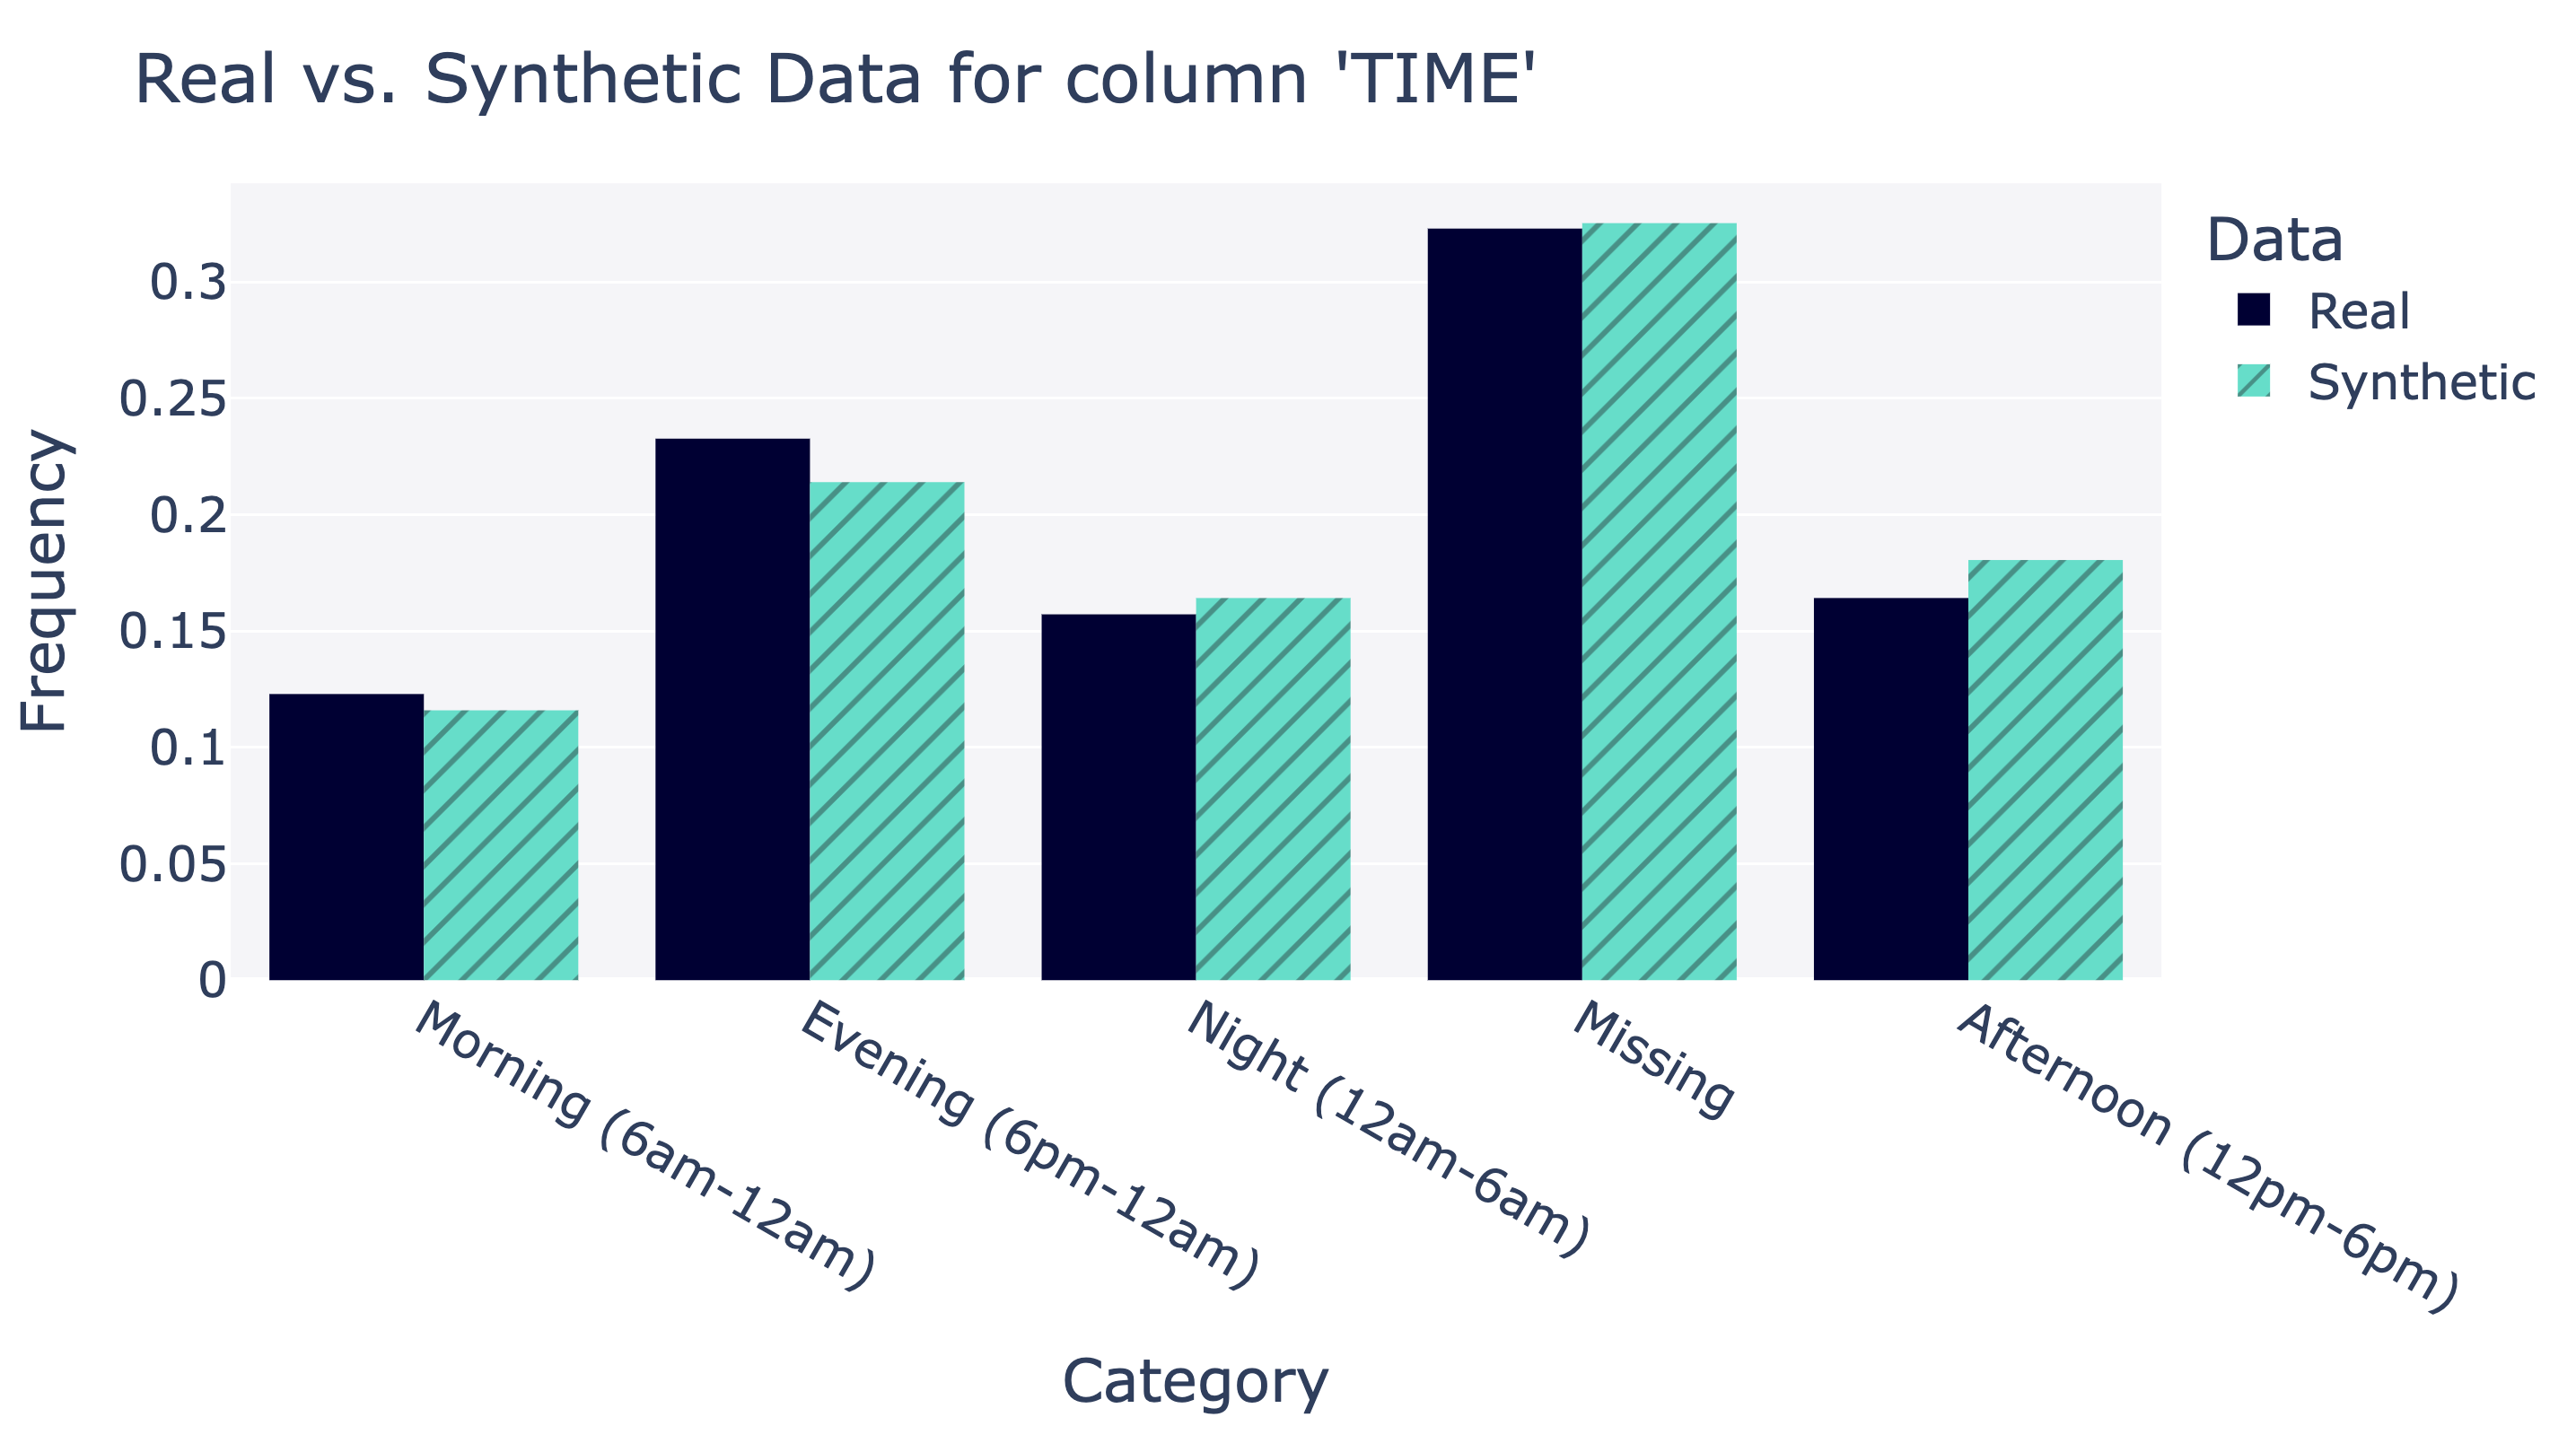
\includegraphics[width=0.8\textwidth]{Images/timefirst.png}
    \caption{Example of a synthesized variable with high quality score}
    \label{fig:proof_1}
\end{figure}
\vspace{10pt}

However, the univariate distribution in other variables, such as the judicial process, was significantly worse and below the desired threshold.

\vspace{10pt}
\begin{figure}[h!]
    \centering
    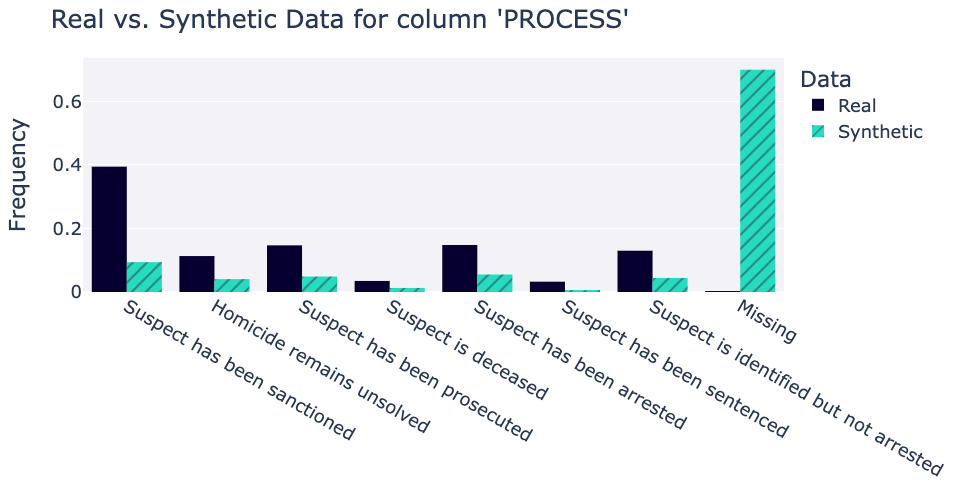
\includegraphics[width=0.8\textwidth]{Images/SENSYN_badsyn1.png}
    \caption{Example of a synthesized variable with low quality score}
    \label{fig:proof_1}
\end{figure}
\vspace{10pt}

Similarly, significant limitations are visible in the bivariate distributions, that is the relationship between variables.

\vspace{10pt}
\begin{figure}[h!]
    \centering
    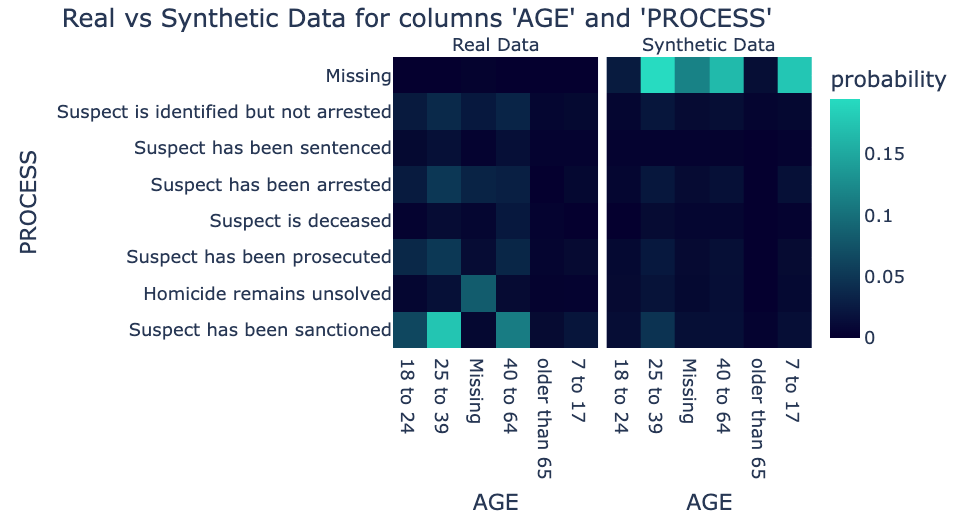
\includegraphics[width=0.8\textwidth]{Images/SENSYN_biva1.png}
    \caption{Example of bivariate relationship comparison across original and synthetic data}
    \label{fig:proof_1}
\end{figure}
\vspace{10pt}

Simply based on these limitations, we concluded that the synthetic dataset did match the requirements set out in the beginning. As such, we did not conduct further analysis, such as replication studies, or an evaluation of the privacy guarantees of the synthetic data.\\


\textbf{Reflections}

After deliberations, we determined two potential causes for the lower than expected quality of the synthetic dataset. First, our data is relatively complex as it spans over three table, meaning that the synthesiser has to learn not only about the patterns and relationships within \textit{one} table (e.g. the relationship between the victim's gender and age) but also across the three tables (e.g. the relationship between type of crime scene, gender of the victim and gender of the perpetrator). In addition, the synthesiser has to replicate relatively many variables (29 divided over the three tables) and many categories within those variables. As mentioned previously, some of the variables have up to 35 categories, with each of these categories having certain patterns and relationships with all the other categories across all variables. Given that about 70 percent of the variables in the synthetic dataset compared well to the original dataset, but the remaining 30 percent did not, we believe that the synthesiser over-corrected, meaning that it tried to mimic as many patterns and relationships as best as possible at the costs of the quality of the patterns and relationships that remained. A second problem that might have impacted the results is that our dataset contains relatively little data, with 1271 cases, information on 1348 victims and 1711 perpetrators. Although this amount is technically sufficient to train a model on the patterns and relationships within that dataset, more data provides a better ground for detecting all underlying patterns and relationships, especially when the data contains many variables as in this case.

Therefore, we decided to address these causes in a second round, meaning that we started again at the step of data preparation.


\subsection{Second attempt}

\textbf{Step 1: Preparations}\\
In order to address the possible causes of the limited data utility in the first attempt, we decided to \textbf{(a)} reduce the complexity of the data as much as possible, and \textbf{(b)} to increase the amount of data.

To reduce the complexity of the data, we decided to minimise both the number of variables, as well as the number of categories within the variables. In total, we excluded six variables: the profession of the victim or perpetrator, whether the victim or perpetrator was under the influence of drugs or alcohol, whether the victim or perpetrator had a violent history, the main motive of the perpetrator and whether the perpetrator committed or attempted suicide. These variables had a significant amount of missing data (and therefore the lowest quality) and were deemed the least important by the project team members with expertise on homicide research. To reduce the number of categories within each variable, we first detected categories with only few cases, such as sexual homicides. After, we aimed to merge these categories together into categories of 'other', based on the number of cases, as well as on logical reasoning. For example, the Dutch Homicide Monitor differentiates between three different types of child homicides: infanticides - the killing of newborns -, the homicide of children by someone in the child's family and the killing of a child by someone outside of the child's family. For the sake of decreasing categories, these three types were merged into one category: \textit{child homicide}. Yet, in order to keep as much detail as possible in the original and thus also the synthetic data, we merged as little categories as deemed necessary at this stage in the process.

To increase the amount of data through which the synthesiser can learn about the patterns and relationships, we decided to broaden the scope of homicide data included, from ten years of homicide data to twenty years of homicide data. As a result, the original dataset used to train the synthesiser now contained 3152 cases, and information on 3358 victims and 4394 perpetrators. \\

\textbf{Step 2: Choosing generation method and tool}\\
The generation method and chosen tool (Synthetic Data Vault) remained the same. However, given that we added new data and recoded some of our variables, we re-run the steps for data cleaning and the preparation of the meta-data.

\begin{figure}[H]
    \centering
    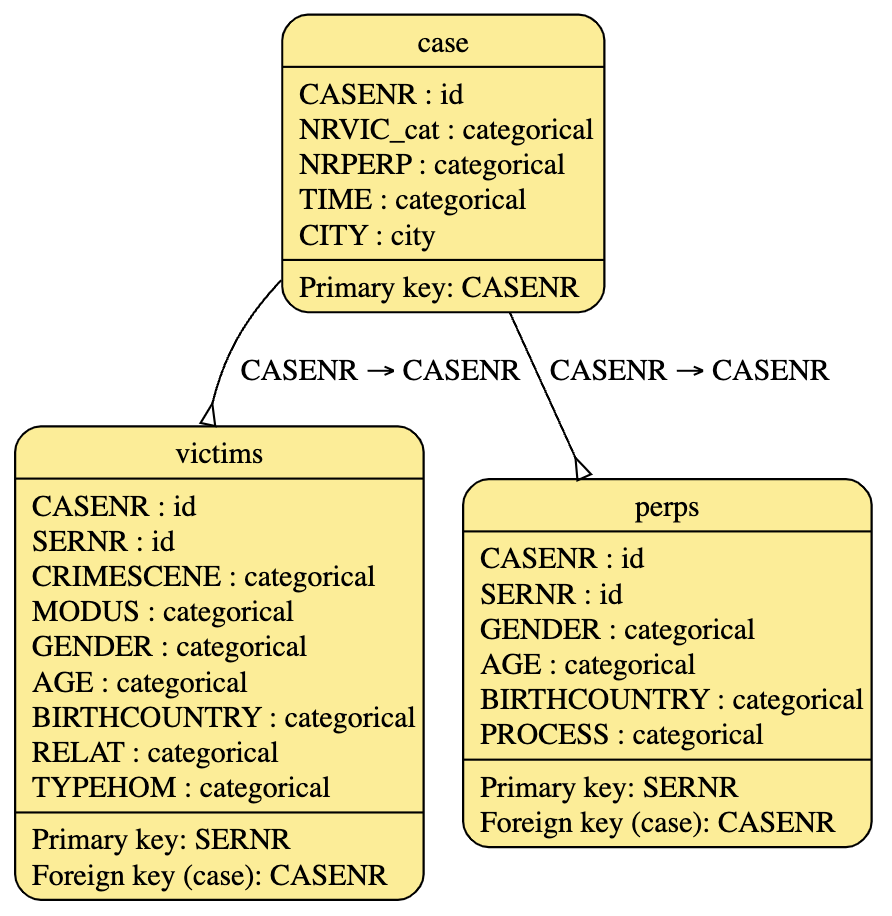
\includegraphics[width=0.8\textwidth]{Images/meta2.png}
    \caption{Dutch Homicide Monitor split into three separate datasets: cases, victims \& perpetrators}
    \label{fig:proof_1}
\end{figure}
\vspace{10pt}


\textbf{Step 3: Generation}\\
As in the previous attempt, we created a synthesiser based on the new meta-data and fed the synthesiser our new dataset to learn the patterns and relationships. Yet, considering that the new adaptions were made in the original dataset, the process and code remained the same.

\newpage
\begin{lstlisting}[caption={Synthetic Data Generation: Second Attempt}, label={lst:gen_first}]
from sdv.multi_table import HMA Synthesizer

synthesizer = HMASynthesizer(metadata, #this creates a model that knows the structure of the original dataset
                             locales=['nl_NL'] #this generates city names in Dutch

synthsizer.add_constraints(constraints=[
    infanticide_constraint, IPH_constraint
])

synthesizer.fit(DHM) #this tells the model to learn from our original dataset
synthetic= synthesizer.sample(scale=1) #this tells the model to create a synthetic dataset with as many rows as the original dataset
\end{lstlisting}
\vspace{10pt}

\textbf{Step 4: Privacy and utility evaluation}\\
With regards to the utility of the data, we detected similar issues as during the first attempt. Again, most of the variables in the synthesised dataset compared well to the original dataset, yet other variables were synthesised poorly. The bivariate relationships of the variables improved compared to the first attempt, yet were still not at a quality that we were satisfied that this synthetic dataset fulfils the statistical requirements set in the beginning. \\

\vspace{10pt}
\begin{table}[H]
\small
\resizebox{\textwidth}{!}{
\begin{tabular}{@{}lll@{}}
\toprule
Quality Type &
  Score (\%) &
  Interpretation \\ \midrule
Data validity &
  100 &
  \begin{tabular}[c]{@{}l@{}}The synthetic data has the same internal structure \\ as the original one\end{tabular} \\
Data structure &
  100 &
  \begin{tabular}[c]{@{}l@{}}The synthetic data has the same columns \\ with the same names\end{tabular} \\
Relationship validity &
  99.99 &
  \begin{tabular}[c]{@{}l@{}}Each case in the victim \& perpetrator datasets \\ are linked to a case in the case dataset\end{tabular} \\
Univariate distribution &
  75.84 &
  \begin{tabular}[c]{@{}l@{}}A variable in the synthetic dataset is on average \\ 75\% similar to the variable in the real dataset\end{tabular} \\
Bivariate distribution within one table &
  51.51 &
  \begin{tabular}[c]{@{}l@{}}The relationship between two variables in the \\ synthetic data is about 50\% similar to the \\ relationship in the real dataset\end{tabular} \\
Structure across tables &
  90.97 &
  \begin{tabular}[c]{@{}l@{}}Around 90\% of cases in the synthetic dataset has the \\ same number of victims and perpetrators associated \\ as in the real dataset\end{tabular} \\
Bivariate distribution across tables &
  63.9 &
  \begin{tabular}[c]{@{}l@{}}The relationship between two variables across \\ the three synthetic datasets is about 64\% similar \\ to the relationship in the real data\end{tabular} \\
Overall &
  70.56 &
  \begin{tabular}[c]{@{}l@{}}Overall, the synthetic dataset compares \\ around 70\% to the real data\end{tabular} \\ \bottomrule
\end{tabular}
}
\caption{General quality report}
\label{tab:my-table}
\end{table}
\vspace{10pt}

\begin{table}[H]
\centering
\small
\begin{tabular}{@{}ll@{}}
\toprule
Variable                                              & Score (\%)   \\ \midrule
Perpetrator birth country                             & 89.87 \\
Status of case against perpetrator in judicial system & 82.36 \\
Perpetrator age                                       & 75.78 \\
Perpetrator gender                                    & 30.5 \\ \bottomrule
\end{tabular}
\caption{Example: quality of each variable in the synthetic perpetrator dataset, ranked from highest to lowest similarity score}
\label{tab:my-table}
\end{table}
\vspace{10pt}


\begin{figure}[H]
\centering
    \hfill
    \subfigure[Example of a synthesised variable with high quality score]{
        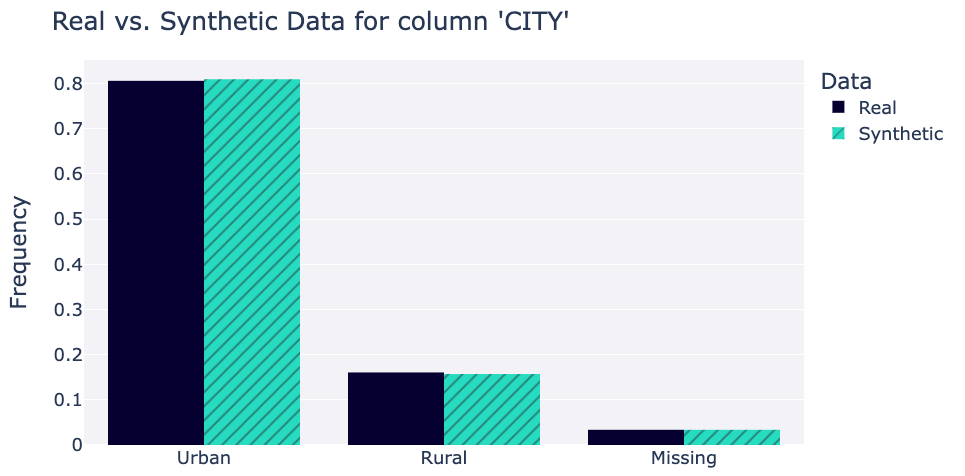
\includegraphics[width=0.8\textwidth]{Images/SENSYN_good2.png}
        \label{fig:subfig2}
    }
    \hfill
    \subfigure[Example of a synthesised variable with low quality score]{
        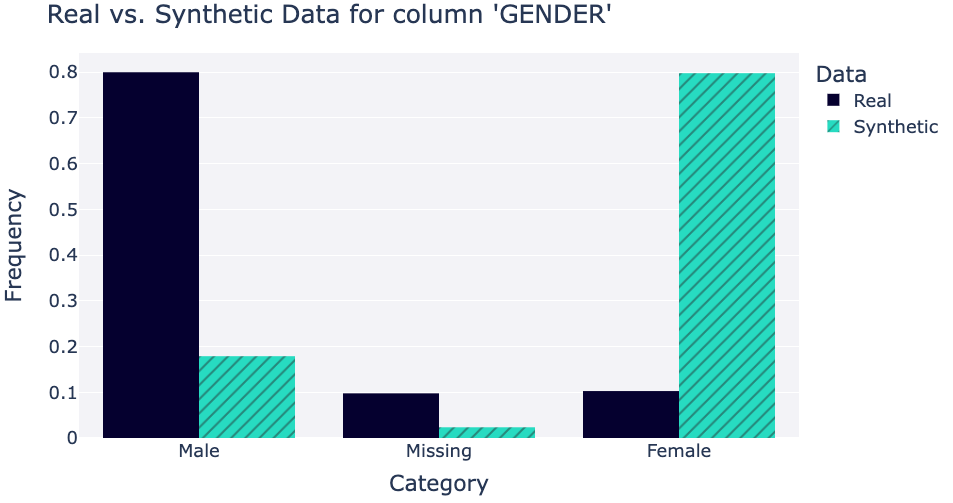
\includegraphics[width=0.8\textwidth]{Images/SENSYN_bad2.png}
        \label{fig:subfig2}
    } 
    \hfill
    \subfigure[Example of bivariate relationship comparison across original and synthetic data]{
        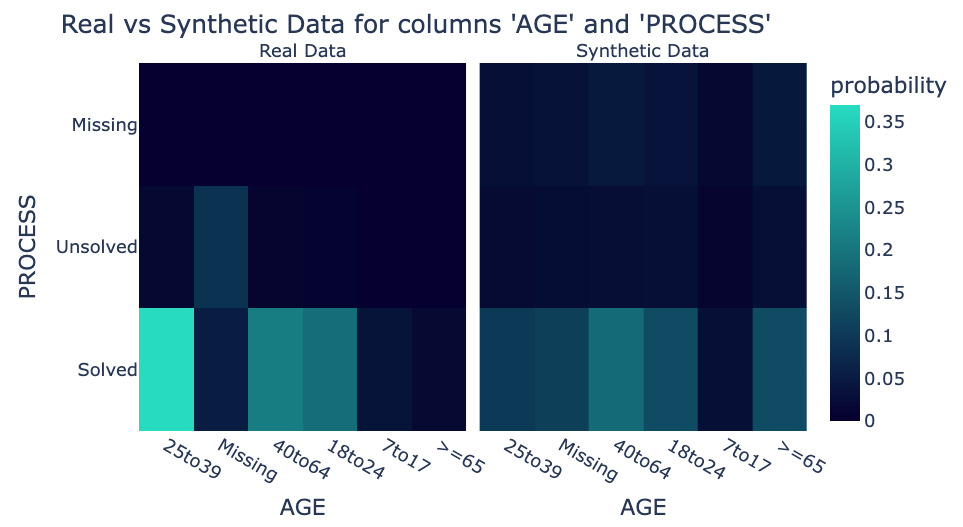
\includegraphics[width=0.8\textwidth]{Images/SENSYN_biva2.png}
        \label{fig:subfig2}
    }
    \caption{Quality of the second synthetic version of the DHM (continued)}
    \label{fig:main_fig}
\end{figure}


Again, we did not conduct any privacy analyses due to the low level of utility.\\

\textbf{Reflections}

Going back to the potential causes of the limited quality, we concluded that the increased amount of data had little impact on the quality of the synthetic dataset. Instead, we had to again review how to reduce the complexity in our data.

Initially, we followed the same procedure as in our previous attempt, by merging categories within variables wherever logically possible. For example, the variable on victim-perpetrator relationship went from 35 categories to only ten categories.

Unfortunately, although the quality of the synthetic dataset improved slightly with each merging, it did not reach a level of quality that was satisfying. Moreover, at a certain point, even further merging of the variables would have significantly changed the level of detail in the dataset, which is one of the main advantages of the original Dutch Homicide Monitor.

\subsection{Final attempt}

\textbf{Step 1: Preparations}\\
With this conclusion in mind, we decided to reduce the complexity, by reducing the multi-table approach to a single-table approach in which the synthesiser only has to recognise the patterns and relationships across one table instead of three. This meant that we had to merge the three tables with the original data (case table, victim table and perpetrator table) back into one single table. With the original structure, the synthesiser would be able to learn the dependencies across the rows, thus individuals that are involved as either victim or perpetrator in the same case. As such, we had to concede that we would not be able to create a synthetic dataset that would allow analysis on the level of case, victim \textbf{and} perpetrator. Based on domain expertise, we decided to merge the information of the main perpetrator onto the row of each associated victim and add a variable that would define one main victim per case. As a result, all information on each individual case and each individual victim is kept in the dataset, yet information for some perpetrators (specifically in cases with multiple perpetrators) were lost. In addition, to increase the quality of the remaining data, we decided to again only use homicide data of ten years as this is the most complete data in the original dataset. Finally, we also reverted most of the merging of categories within the variables, in order to keep as much detail as possible.

\textbf{Step 2: Choosing generation method and tool}] \\
Given the changed structure of the original dataset, we had to revisit the requirements of the Synthetic Data Vault for single table synthesis. In essence, only few changes had to be made, in particular with regards to the meta-data.

\vspace{10pt}
\begin{figure}[H]
    \centering  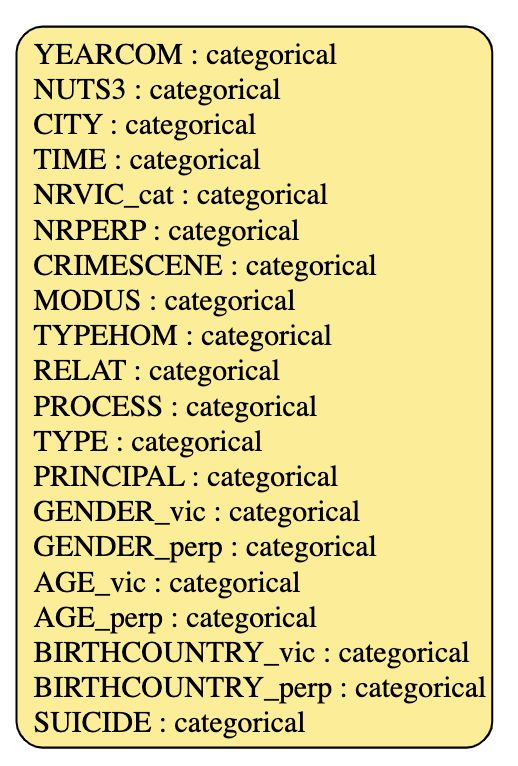
\includegraphics[width=0.5\textwidth]{Images/meta3.png}
    \caption{Dutch Homicide Monitor as one dataset, with each row representing one victim}
    \label{fig:proof_1}
\end{figure}
\vspace{10pt}

\textbf{Step 3: Generation} \\
As in the previous steps, we used the meta-data of the single table with homicide information to create a synthesiser, and trained said synthesiser with the original dataset.

\vspace{10pt}
\begin{lstlisting}[caption={Synthetic Data Generation: Final Attempt}, label={lst:gen_first}]
from sdv.single_table import GaussianCopulaSynthesizer

synthesizer = GaussianCopulaSynthesizer(metadata,
                                        locales=['nl_NL']

synthesizer.add_constraints([IPHConstraint,kindermoordConstraint])

synthesizer.fit(DHM)
synthetic=synthesizer.sample(num_rows=1364)
\end{lstlisting}
\vspace{10pt}

\textbf{Step 4: Privacy and Utility Evaluation}

In this attempt, both the comparison of the univariate as well as bivariate patterns between the original and synthetic data looked significantly improved, which is supported by the quality report provided by the Synthetic Data Vault package.

\vspace{10pt}
\begin{table}[H]
\small
\resizebox{\textwidth}{!}{
\begin{tabular}{@{}lll@{}}
\toprule
Quality Type &
  Score (\%) &
  Interpretation \\ \midrule
Data validity &
  100 &
  \begin{tabular}[c]{@{}l@{}}The synthetic data has the same internal structure \\ as the original one\end{tabular} \\
Data structure &
  100 &
  \begin{tabular}[c]{@{}l@{}}The synthetic data has the same columns \\ with the same names\end{tabular} \\
Univariate distribution &
  97.8 &
  \begin{tabular}[c]{@{}l@{}}A variable in the synthetic dataset is on average \\ 98\% similar to the variable in the real dataset\end{tabular} \\
Bivariate distribution within one table &
  89.67 &
  \begin{tabular}[c]{@{}l@{}}The relationship between two variables in the \\ synthetic data is about 90\% similar to the \\ relationship in the real dataset\end{tabular} \\
Overall &
  93.74 &
  \begin{tabular}[c]{@{}l@{}}Overall, the synthetic dataset compares \\ around 94\% to the real data\end{tabular} \\ \bottomrule
\end{tabular}
}
\caption{General quality report}
\label{tab:my-table}
\end{table}
\vspace{10pt}

\begin{table}[H]
\centering
\small
\begin{tabular}{@{}ll@{}}
\toprule
Variable                                              & Score (\%)   \\ \midrule
Type: victim or perpetrator?                          & 99.93 \\
City homicide was committed in                        & 99.79 \\
Number of perpetrators                                & 99.21 \\
Status of case against perpetrator in judicial system & 99.13 \\
Number of victims                                     & 98.98 \\
Time of day homicide was committed                    & 98.87 \\
Perpetrator gender                                    & 98.81 \\
Perpetrator birthcountry                              & 98.3  \\
Type of crimescene                                    & 98.04 \\
Victim gender                                         & 97.9  \\
Victim age                                            & 97.38 \\
Perpetrator age                                       & 97.32 \\
Modus operandi                                        & 97.11 \\
Victim-perpetrator relationship                       & 96.95 \\
Victim birthcountry                                   & 96.89 \\
Year homicide was committed                           & 95.2  \\ 
Region homicide was committed                         & 94.92 \\
Context of homicide                                   & 93.53 \\ \bottomrule
\end{tabular}
\caption{Quality of each variable in the synthetic dataset, ranked from highest to lowest similarity score}
\label{tab:my-table}
\end{table}

\begin{figure}[H]
    \hfill
    \subfigure[Example of a synthesised variable with high quality score]{
        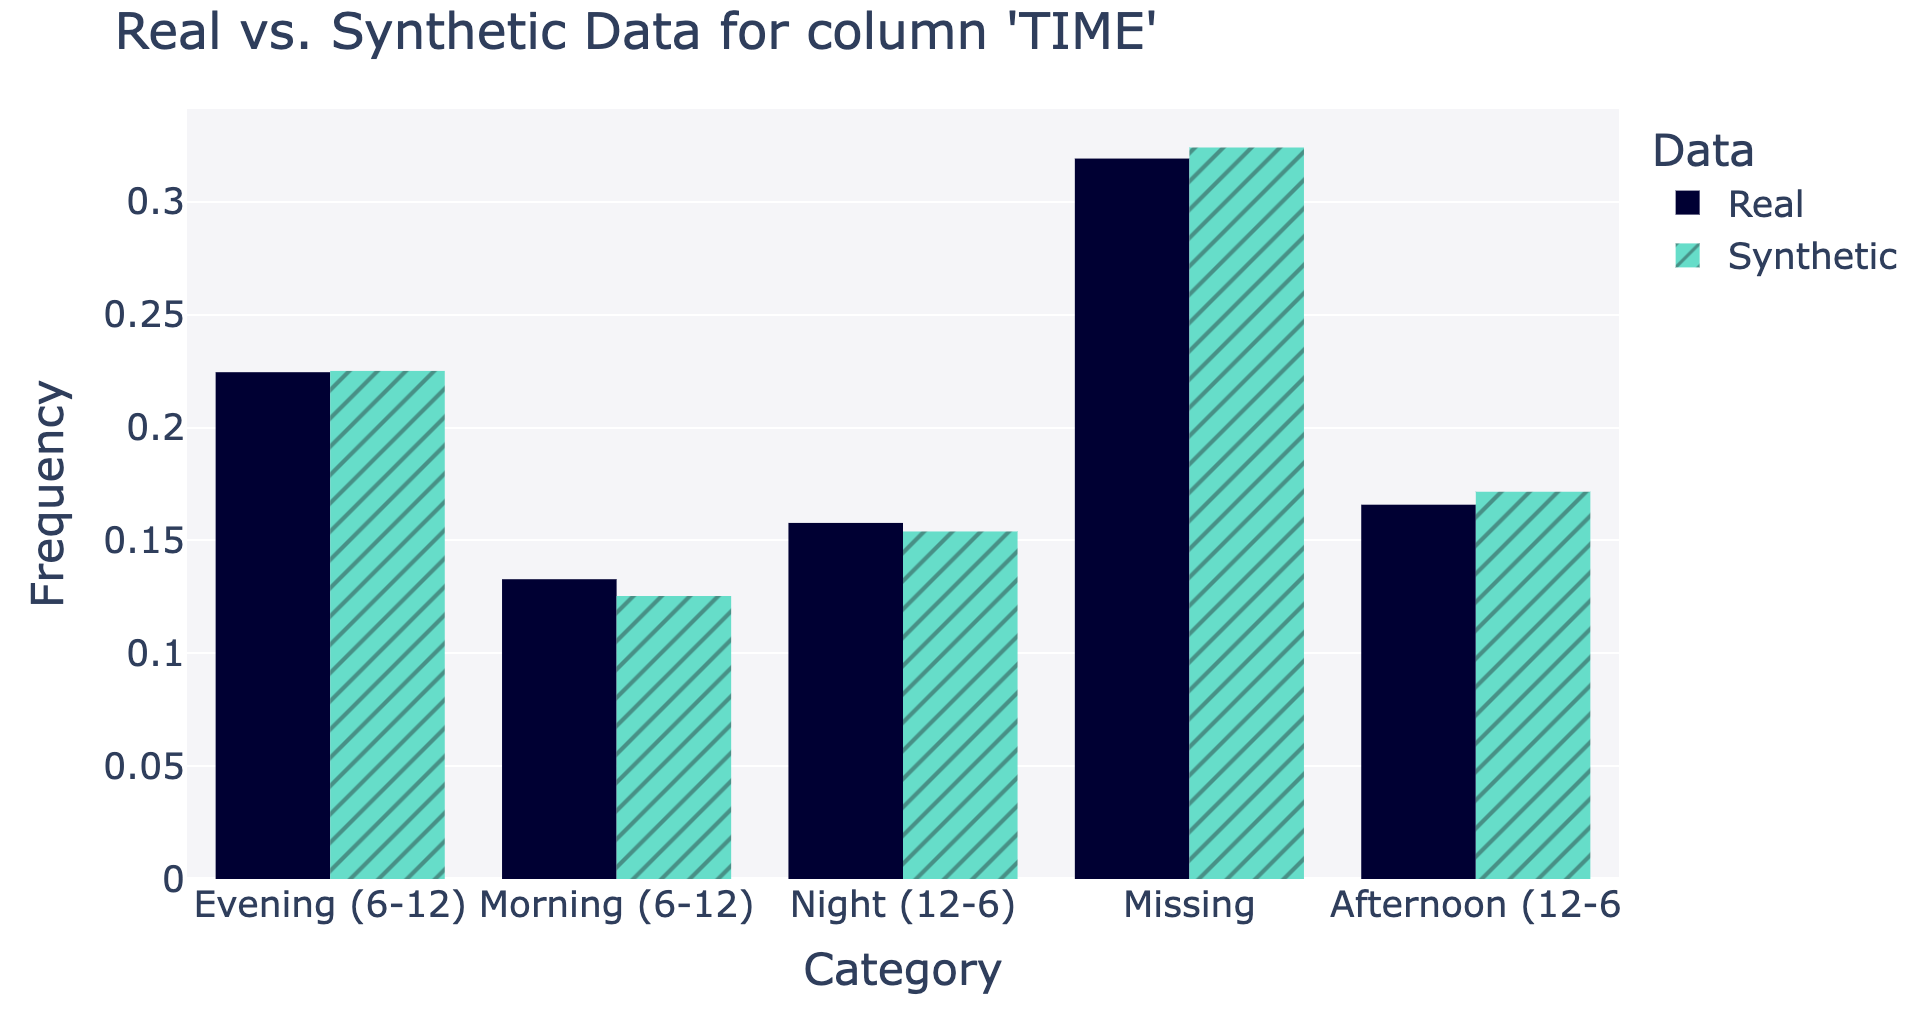
\includegraphics[width=0.8\textwidth]{Images/SENSYN_goodFINAL.png}
        \label{fig:subfig2}
    }
    \hfill
    \subfigure[Example of a synthesised variable with the lowest quality score]{
        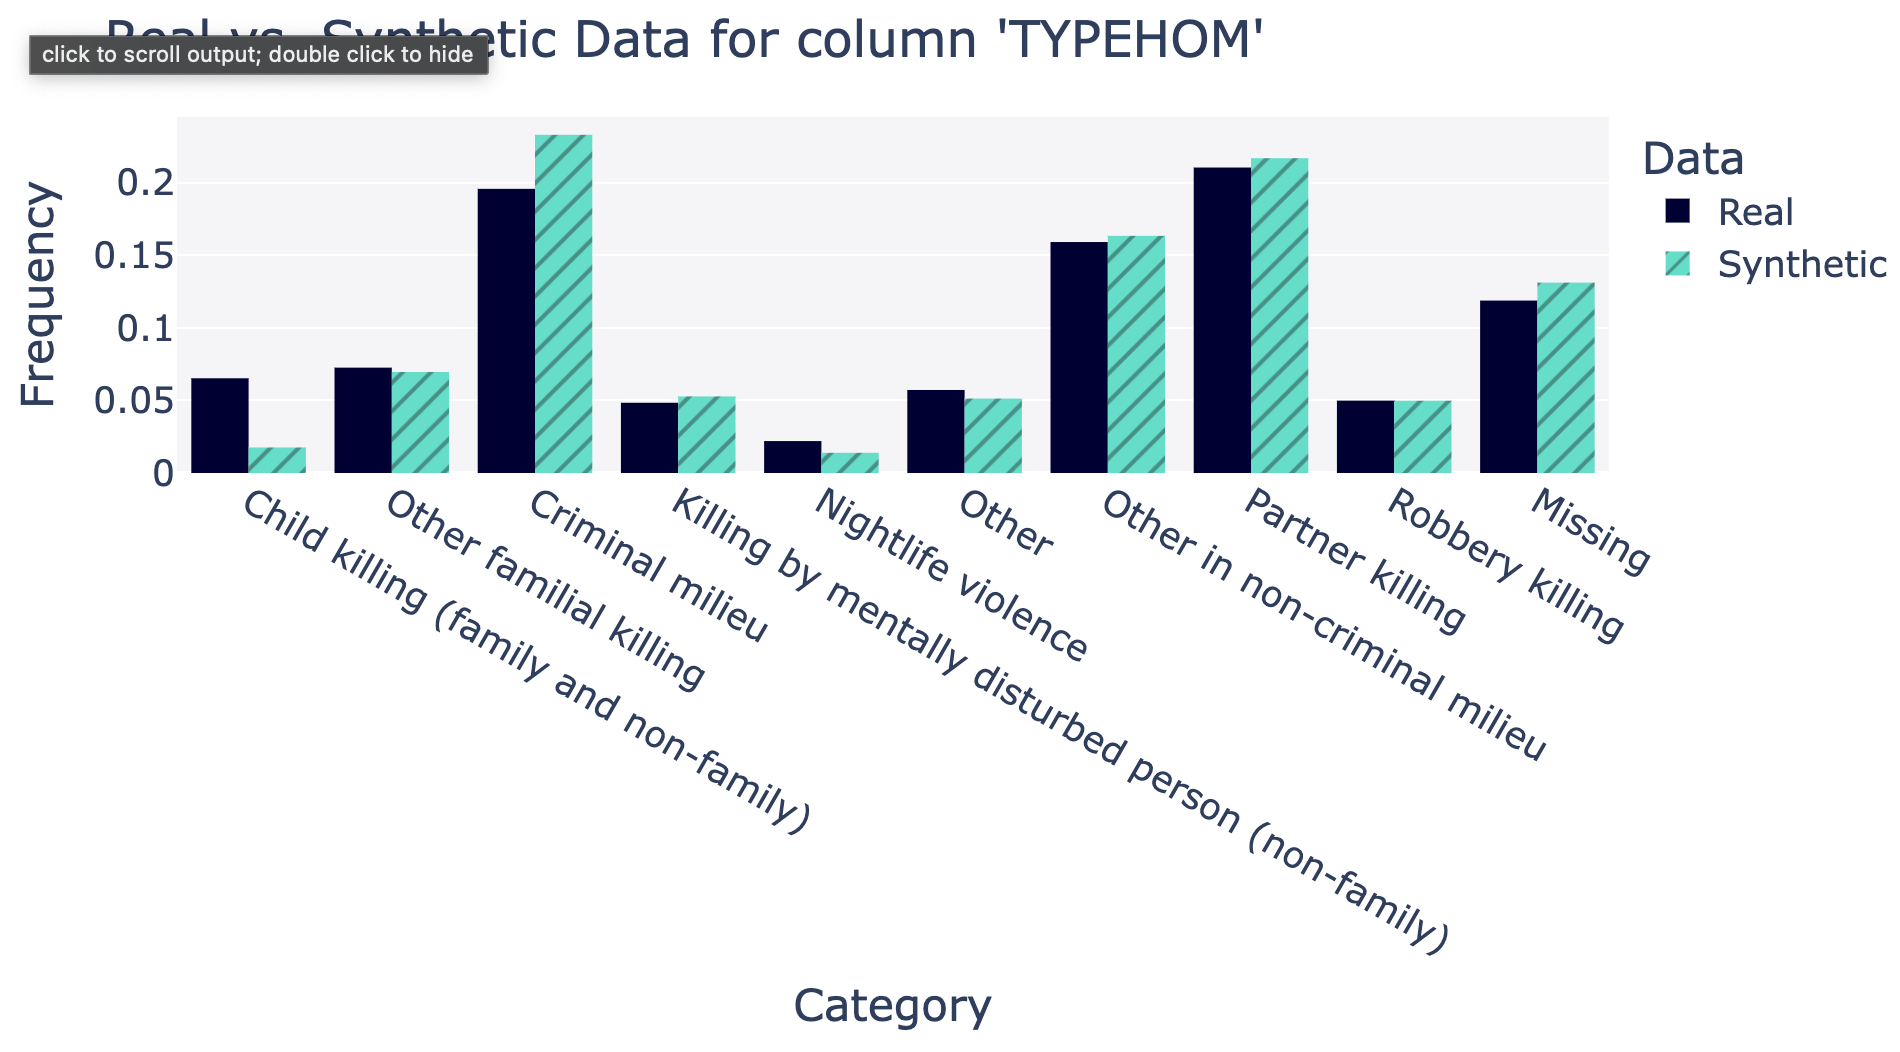
\includegraphics[width=0.8\textwidth]{Images/SENSYN_badFINAL.png}
        \label{fig:subfig2}
    }
    \centering
    \hfill
    \subfigure[Example of bivariate relationship comparison across original and synthetic data]{
        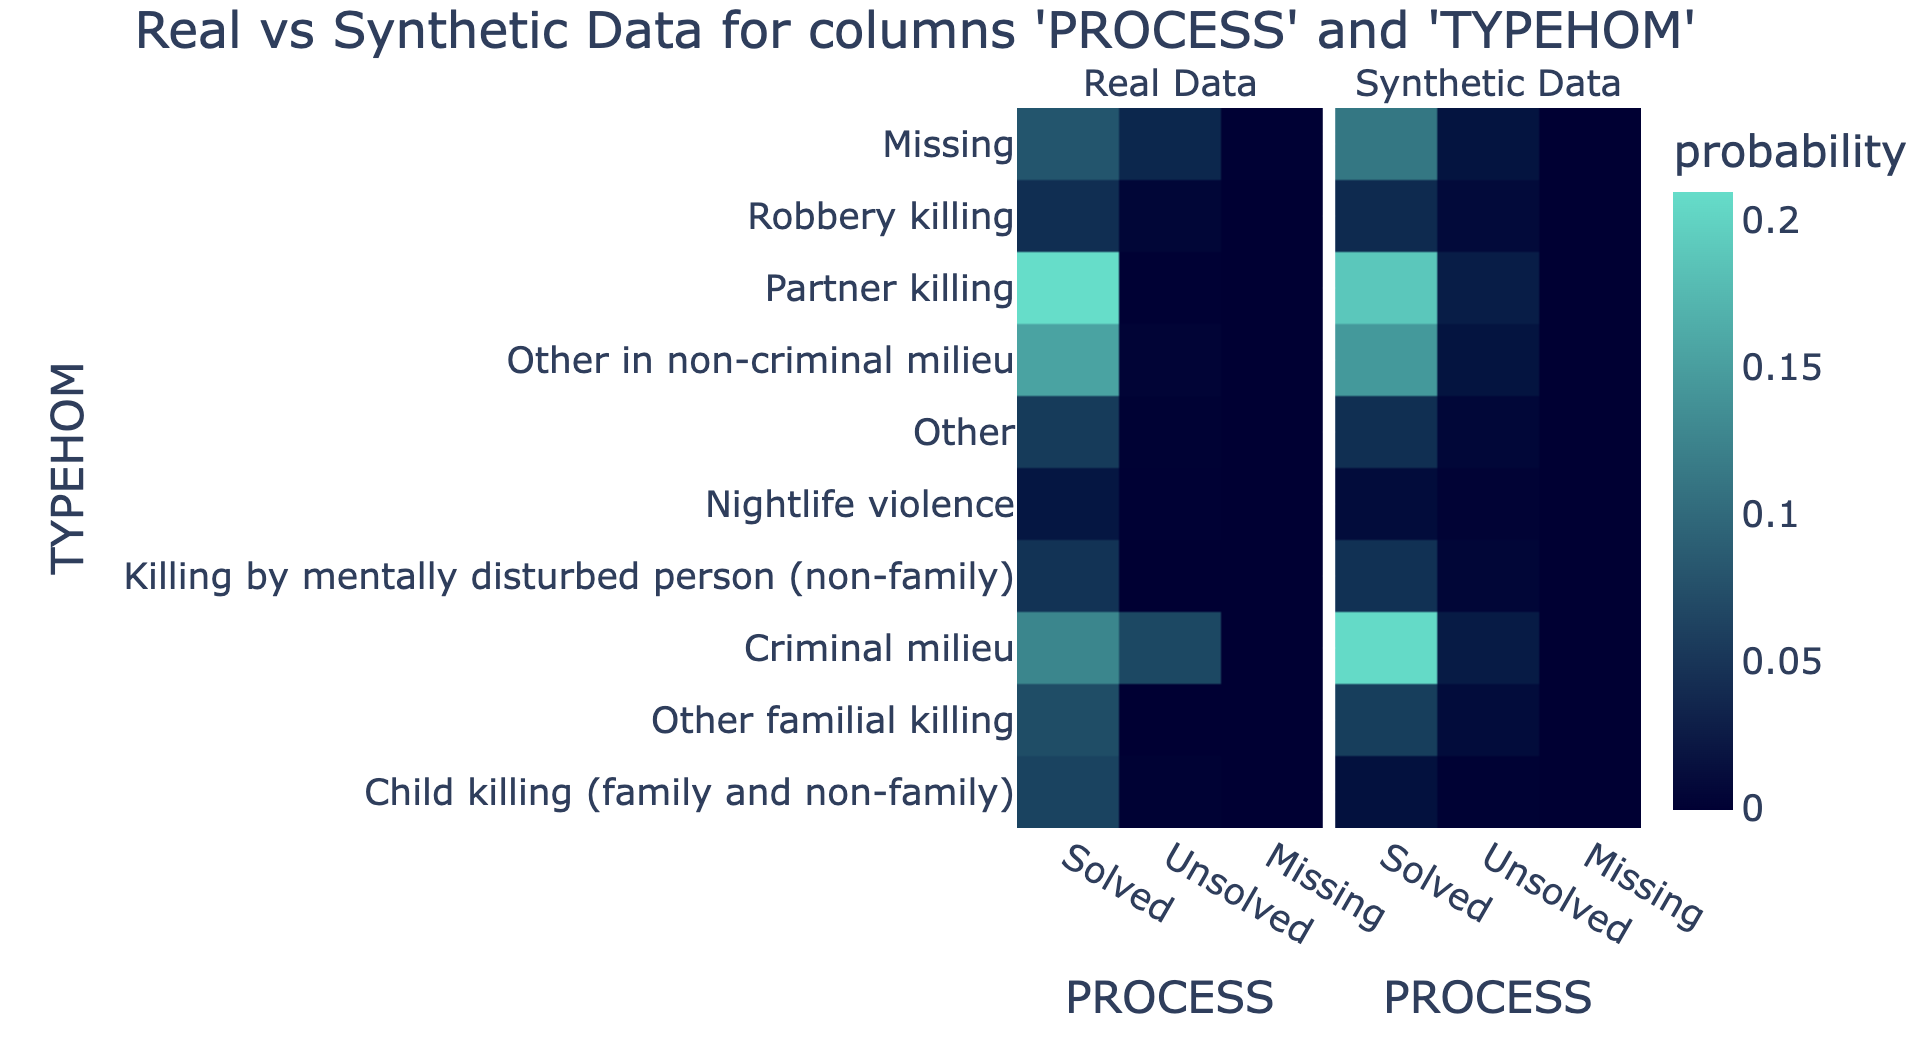
\includegraphics[width=0.8\textwidth]{Images/SENSYN_bivaFINAL.png}
        \label{fig:subfig2}
    }
    \caption{Quality of the final synthetic version of the DHM (continued)}
    \label{fig:main_fig}
\end{figure}
\clearpage

To check the extent of the statistical accuracy of the synthetic dataset, we conducted two replication studies, based on studies previously conducted with the original data. Although the previous studies used homicide data for different years, we expected the results to be similar with the ten year of homicide data included in the synthetic data. Our expectations were (mostly) met: \\
\hl{add example study 1}

Overall, this synthetic version of the Dutch Homicide Monitor satisfied our requirements with regards to data utility.

With regards to data privacy, we conducted several tests to check whether the safeguarding of sensitive and personal data is equally satisfying. First, we randomly selected about twenty cases from the original dataset and tried to identify cases that match their profiles in the synthetic dataset. In addition, we identified certain outliers in the original dataset, e.g. individuals with unusual combination of attributes, and tested whether we were able to identify similar cases in the synthetic dataset.
In both cases, were not able to detect one-on-one matches between the original and synthetic dataset with our chosen sample and outliers. Finally, we used privacy-metrics included in the SDV-package, the so-called \textit{Privacy Against Inference} metrics. These metrics calculate the risk of an attacker learning sensitive information based on the synthetic dataset, assuming that the attacker already has some information based on real data. The metrics allow for a simulation of this risk with all possible variable combinations.

\vspace{10pt}
\begin{lstlisting}[caption={SDV privacy metrics example}, label={lst:gen_first}]
from sdmetrics.single_table import CategoricalKNN,CategoricalRF

CategoricalKNN.compute(
    real_data=case,
    synthetic_data=synthetic,
    key_fields=['GENDER_vic','CRIMESCENE'], #these are the variables we assume the attacker already knows
    sensitive_fields=['RELAT'] #this is the variable the attacker wants to know
\end{lstlisting}
\vspace{10pt}

For each variable-combination, the algorithms provides a percentage; 0\% means that the data is not safe at all, 100\% means that the data is completely safe. In the example in the listing above, the information about the victim-perpetrator relationship was 79.7\% safe, given that the attacker already knows the victim's gender and the type of crimescene.

%%%%%%%%%%%%%%%%%%%%%%%%%%%%%%%%%%%%%%%%

\section{Concluding Reflections}

\subsection{The Process}
Taking into account data preparation and necessary adaptions for each cycle, the overall process only took about two full days; the actual generation of the synthetic data between a few seconds for final single table to a few minutes for the most complex multi-table. Moreover, through the detailed documentation provided by the Synthetic Data Vault library, as well as a helpful community of users online, any questions or problems along the process have quickly been answered or solved. In addition, the synthesis of data with the use of the Synthetic Data Vault has proven very accessible, even for someone without extensive knowledge of programming or synthetic data. 

\subsection{The Data}
In the beginning of the process, we set high aims and requirements for the synthetic version of the Dutch Homicide Monitor. In simple terms, we wanted to create a synthetic dataset that mimics the original data enough to be used for advanced scientific analysis, to be informative for non-scientific purposes but to safeguard the privacy of all individuals included in the dataset. In the end, not all of the requirements have been met, in particular the requirement that the full original dataset had to be synthesised. Due to the complexity of the original data impacting the quality of the synthetic data, we had to opt to exclude information on certain perpetrators (in cases in which there were more than one perpetrator). Thus, information from the original dataset was lost during the process. The final synthetic dataset, however, provides a good balance between privacy assurance and data quality. 

\subsection{Open \& FAIR data}
\hl{add}
With regards to open science principles, the synthetic dataset has been developed with the FAIR principles in mind. Therefore, the full disaggregated data can be found, used and downloaded at the projects webpage \hl{add link}
\hl{add screenshot webpage}




